\chapter{Wstęp}

\section{Cassandra}

Apache Cassandra to darmowa, rozproszona baza danych przeznaczona do zarządzania dużymi ilościami ustrukturyzowanych danych. Projekt powstał, aby umożliwić realizację funkcjonalności przeszukiwania skrzynki odbiorczej użytkownika na portalu Facebook\footnote{Popularny portal społecznościowy dostępny pod adresem \url{http://fb.com}.}. Funkcjonalność ta nie była możliwa do zrealizowania w~oparciu o~tradycyjny, relacyjny model bazy danych. W~2008 Facebook udostępnił kod źródłowy Cassandry, która następnie (w~2010 roku) została wcielona do projektów pod opieką fundacji Apache\footnote{Fundacja wspierająca powstawanie oprogramowania o~otwartym źródle.}.\cite{casshistory} 

Apache Cassandra jest częścią ruchu NoSQL\footnote{NoSQL - \emph{Not only SQL} (ang. nie tylko SQL).}. Chociaż brakuje oficjalnej, ustanowionej odgórnie definicji pojęcia NoSQL możemy wyróżnić zestaw cech wspólnych baz danych, które powszechnie zaliczane są do tej grupy:

\begin{itemize}
	\item Wewnętrzna reprezentacja danych w~bazach NoSQL nie opiera się na tabelach i~relacjach.
	\item Brak pełnej implementacji języka SQL. Chociaż niektóre bazy NoSQL wykorzystują język zapytań o~składni podobnej do SQL, żadna z~nich nie implementuje jej w~pełni.
	\item Bazy NoSQL posiadają elastyczny model danych. Nie wykorzystują sztywnego, narzuconego z~góry schematu.
	\item Model danych w~bazach NoSQL jest zazwyczaj ukierunkowany na łatwe klastrowanie, chociaż istnieją wyjątki od tej reguły (na przykład Neo4j\footnote{Neo4j - baza danych oparta wewnętrznie o~grafy.}).
	\item Bazy NoSQL są przystosowane do wymagań nowoczesnych portali internetowych, które muszą obsługiwać ogromne zbiory danych z~szybkim czasem dostępu. \cite{nosqldistilled}
\end{itemize}

Konsekwencją ostatniej cechy jest odejście od idei właściwości ACID. Zestaw cech ACID\footnote{ACID - skrót od \emph{Atomicity, Consistency, Isolation, Durability} (ang. atomowość, jednorodność, izolacja, trwałość)} to minimalny zbiór cech, które gwarantują realizację transakcyjności w~bazie danych. \cite{transactionconcept} Klastrowanie sprawia, że nie da się zachować spójności danych na wszystkich węzłach, stąd wymagane są inne mechanizmy zachowania poprawności danych.

\section{Historia Cassandry}

Apache Cassandra powstała z~połączenia rozwiązań wykorzystywanych w~dwóch mechanizmach bazodanowych: Google Bigtable oraz Amazon Dynamo. Google Bigtable to rozproszony system bazodanowy do przechowywania ustrukturyzowanych danych. Został stworzony z~myślą o~skalowaniu dla ogromnych ilości danych. Wykorzystywany jest między innymi w~takich produktach jak Google Analytics, Google Finance, Google Earth oraz mechanizmach takich jak spersonalizowane wyszukiwanie w~przeglądarce Google. 

Model danych w~Google Bigtable jest opisany trójwymiarową strukturą mapy. Mapa ta jest identyfikowana unikalnymi kluczami, które reprezentują klucz wiersza, nazwę (klucz) kolumny oraz znacznik czasu. Wszystkie wiersze są uporządkowane w~rosnącym porządku leksykograficznym względem klucza. W~każdej komórce mapy przechowywane są wartości w~postaci łańcucha znaków, co implikuje konieczność serializacji i~deserializacji wartości w~aplikacjach klienckich. Dodatkowo, nazwy kolumn mogą być grupowane w~rodziny. Nazwa każdej kolumny w~rodzinie jest poprzedzona klasyfikatorem, który identyfikuje tę rodzinę (w~formacie \emph{rodzina:nazwa\_kolumny}). \cite{googlebigtable} Schematyczny rysunek przykładowej struktury danych przedstawiono na rysunku \ref{fig:bigtabledatamodel}.

\begin{figure}[ht!]
	\centering
	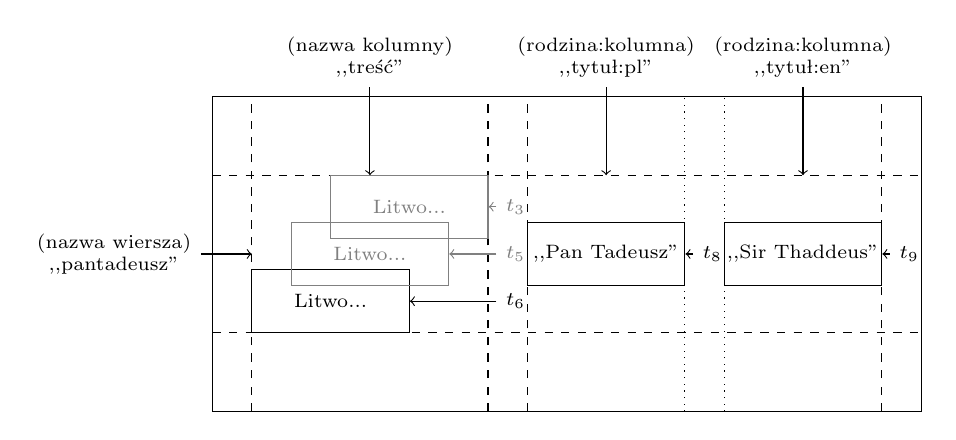
\begin{tikzpicture}
		\draw (0, 0) rectangle (9, 4);
		\draw[style=dashed] (0.5, 0) -- (0.5, 4);
		\draw[style=dashed] (0, 1) -- (9, 1);
		\draw[style=dashed] (0, 3) -- (9, 3);
		\draw[style=dashed] (3.5, 0) -- (3.5, 4);
		\draw[style=dashed] (4, 0) -- (4, 4);
		\draw[style=dotted] (6, 0) -- (6, 4);
		\draw[style=dotted] (6.5, 0) -- (6.5, 4);
		\draw[style=dashed] (8.5, 0) -- (8.5, 4);
		\node[font=\scriptsize, align=center] (content) at (2, 4.5) {(nazwa kolumny) \\ ,,treść''};
		\node[font=\scriptsize, align=center] (polish) at (5, 4.5) {(rodzina:kolumna) \\ ,,tytuł:pl''};
		\node[font=\scriptsize, align=center] (english) at (7.5, 4.5) {(rodzina:kolumna) \\ ,,tytuł:en''};
		\node[rectangle, text=black, draw=black, minimum width=2cm, minimum height=0.8cm, font=\scriptsize, inner sep=0mm] (contentt6) at (1.5, 1.4) { Litwo... };
		\node[rectangle, text=gray, draw=gray, minimum width=2cm, minimum height=0.8cm, font=\scriptsize, inner sep=0mm] (contentt5) at (2.0, 2.0) { Litwo... };
		\node[rectangle, text=gray, draw=gray, minimum width=2cm, minimum height=0.8cm, font=\scriptsize, inner sep=0mm] (contentt3) at (2.5, 2.6) { Litwo... };
		\node[rectangle, text=black, draw=black, minimum width=2cm, minimum height=0.8cm, font=\scriptsize, inner sep=0mm] (titlepolish) at (5, 2.0) { ,,Pan Tadeusz'' };
		\node[rectangle, text=black, draw=black, minimum width=2cm, minimum height=0.8cm, font=\scriptsize, inner sep=0mm] (titleenglish) at (7.5, 2.0) { ,,Sir Thaddeus'' };
		\node[font=\scriptsize, align=center] (rowkey) at (-1.25, 2) {(nazwa wiersza) \\ ,,pantadeusz''};
		\node[font=\scriptsize, align=center] (t6) at (3.85, 1.4) {$t_{6}$};
		\node[font=\scriptsize, align=center, text=gray] (t5) at (3.85, 2.0) {$t_{5}$};
		\node[font=\scriptsize, align=center, text=gray] (t3) at (3.85, 2.6) {$t_{3}$};
		\node[font=\scriptsize, align=center] (t8) at (6.35, 2) {$t_{8}$};
		\node[font=\scriptsize, align=center] (t9) at (8.85, 2) {$t_{9}$};
		\draw[->] (rowkey) -- (0.5, 2);
		\draw[->] (content) -- (2.0, 3);
		\draw[->] (polish) -- (5.0, 3);
		\draw[->] (english) -- (7.5, 3);
		\draw[->, draw=gray] (t3) -- (contentt3);
		\draw[->, draw=gray] (t5) -- (contentt5);
		\draw[->] (t6) -- (contentt6);
		\draw[->] (t8) -- (titlepolish);
		\draw[->] (t9) -- (titleenglish);
	\end{tikzpicture}
	\caption{Schematyczne przedstawienie modelu danych dla Google Bigtable na przykładzie fragmentu danych książek.}
	\label{fig:bigtabledatamodel}
\end{figure}

\section{Architektura}

Placeholder.
